\documentclass[letterpaper]{article}
\usepackage{aaai17}
\usepackage{times}
\usepackage{helvet}
\usepackage{courier}
\usepackage{url}
\usepackage{graphicx}
\usepackage{algorithmicx}
\usepackage{algorithm}
\usepackage[noend]{algpseudocode}
\usepackage{amsmath}
\usepackage{caption}

\graphicspath{{Figures/}}

\frenchspacing
% Add additional packages here. The following
% packages may NOT be used  (this list
% is not exhaustive:
% authblk, caption, CJK, float, fullpage, geometry, 
%hyperref, layout, nameref, natbib, savetrees, 
%setspace, titlesec, tocbibind, ulem
%
%
\begin{document}

%US Lettersize Paper Is Required
\setlength{pdfpagewidth}{8.5in}
\setlength{pdfpageheight}{11in}\\
%
%
% PDFINFO
% You are required to complete the following
% for pass-through to the PDF. 
% No LaTeX commands of any kind may be
% entered. The parentheses and spaces 
% are an integral part of the 
% pdfinfo script and must not be removed.
%
\pdfinfo{
/Title (Input Your Paper Title Here)
/Author (John Doe, Jane Doe)
/Keywords (Input your keywords in this optional area)
}

\title{Intelligent Agents in a Probabilitsic Game : Proximity}
\author{Matthias Denu \and Donald Hamnett\\ 
Northeastern University \\ College of Computer and Information Science\\ 440 Huntington Ave \#202, Boston, MA 02115}

\maketitle 
\begin{abstract}
\par
The aim of this project was to implement intelligent agents to defeat a greedy agent in the game of Proximity.
%...
\end{abstract}
\section{Introduction}
\par

\subsection{Background}
Artificial Neural Networks have their origins in 1943, with the McCollough-Pitts Threshold Logic Unit (TLU), a mathematical interpretation how formal logic is carried out in the human brain.%CITE
The TLU representation of a neuron, is as a unit that takes in a set of inputs and calculates a weighted sum. This weighted sum 
would then be processed as:
\[ 
	f(\mathbf{x}) = \begin{cases}
		0,& \big(\sum\limits_{i}w_ix_i\big) + b < \text{threshhold}\\
		1,  &\text{Otherwise}
		\end{cases}
\]
\captionof{figure}{TLU Activation}
Any discrete binary task could be represented by these units, but their usefulness was simply as a model of the brain and offered no deductive 
improvements upon formal logic.
\begin{figure}[H]
	\centering
	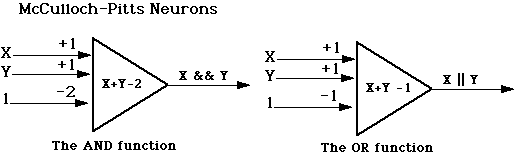
\includegraphics[width=6cm]{mpneuron.png}
	\caption{The McCollough-Pitts Neuron}
\end{figure}
%figure
\par
In 1958, the precursor of the modern-day neural network was born with Rosenblatt's development of the "perceptron."
%cite 
Expanding on the MuCollough-Pitts representation of a neuron, his perceptron was a unit that similarly took in a set of inputs and calculated a weighted sum, activating with the sign function.  
\[ 
	sgn(\mathbf{x}) = \begin{cases}
		-1,& \big(\sum\limits_{i}w_ix_i\big) + b < 0\\
		+1,  &\text{Otherwise}
		\end{cases}
\]
\captionof{figure}{The Sign Function}
The key insight of Rosenblatt was that opposed to weights being fixed, they were adjustable parameters with positive and negative weights, and could hence be learned.
\begin{figure}[H]
	\centering
	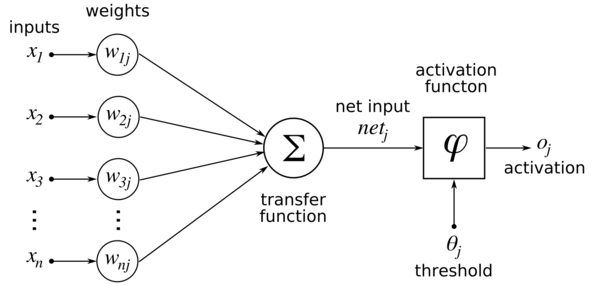
\includegraphics[width=6cm]{Rosenblattperceptron.png}
	\caption{The Rosenblatt Perceptron}
\end{figure}
The full history of perceptrons is outside the scope of this report, but after a period of falling out of fashion, the perceptron has made a massive resurgence in recent years due to the development of the ANN, where several perceptrons are combined in parallel and/or in layers to compute complex 
predictive models that can be applied to non-linearly separable decision boundaries. While the ANN was first developed in the 1960s, notably 
ADALINE and MADELINE, %cite
it was not until the recent increases in both computational power and available data that their widespread use was adopted.
Since then, these networks have had success in a vast collection of problems, ranging from natural language processing with recurrent neural networks, to computer vision with convolutional neural networks (CNNs).  
\par
A convolutional neural network is a popular tool used mainly in image classification and computer vision, but has been applied in recent years to a 
growing number of use cases. The basis of the CNN, and what makes it well suited to computer vision, is the convolutional layers. A convolution in this 
sense is a kernel with trainable weights which has the same depth of the image being convolved (i.e. and RGB image would have a depth of 3). However, 
the other dimensions of this kernel, or "filter," are usually smaller than on the other axes, which allows it to stride across windows of the image. The output 
of a single stride is a scalar, the sum of the element-wise product of the kernel with the input image. Each of these scalars is placed in a new grid, where
spacial relativity of the original image and the kernel outputs are preserved. By using several filters and layers of convolutions (and a lot of training data),
individual kernels can begin to recognize features such as edges and foreground, which when combined can lead to meaningful pattern recognition of the 
images.
\begin{figure}[H]
	\centering
	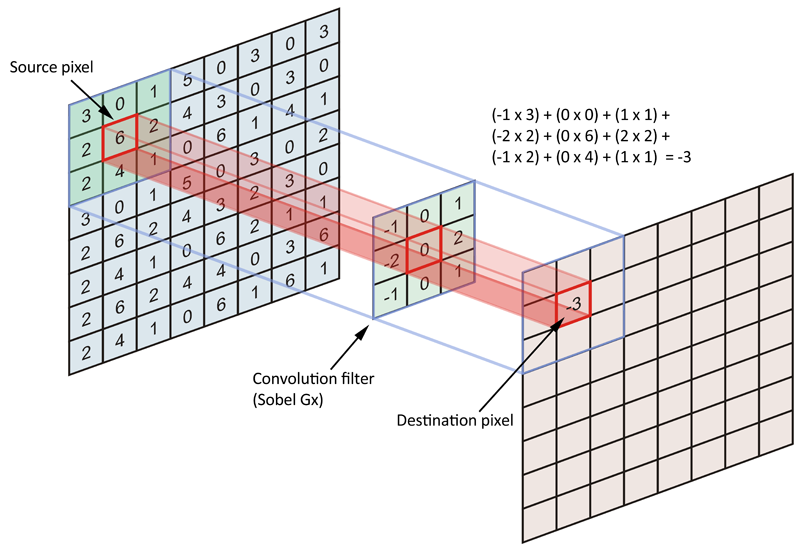
\includegraphics[width=6cm]{convolution.png}
	\caption{A convolution \cite{pjreddie}}
\end{figure}
\subsection{Project Description} 
\par
Using the Keras %cite
deep learning library in Python with its functional API made it incredibly easy to build an ANN. Below is the pseudocode used to build a fully-connected
 feed-forward network.
\begin{algorithmic}[1]
\Procedure{GetNetwork}{NumberOfHiddenLayers}
\State InputLayer $\gets Input($NumberOfFeatures$)$
\State x $\gets$ InputLayer
\For{$i=1$ to NumberOfHiddenLayers} 
        \State x $\gets HiddenLayer($NumberOfFeatures$)$(x)
\EndFor
\State OutputLayer $\gets Layer($1$)$(x)
\State ANN$\gets$ Model(InputLayer, OutputLayer)
\State Compile(ANN) \\
\Return ANN
\EndProcedure
\end{algorithmic}
\par
In all networks, I used the rectified linear unit (ReLU) for the hidden layer activations, and the logistic sigmoid with a threshold of 0.5
 for the output activation.
 \begin{align}
	sigmoid(x) &= \frac{1}{1 + e^{-x}} \\
	ReLU(x) &= \max(0, x)
\end{align}
\captionof{figure}{The sigmoid and ReLU functions}
Below are the relevant parameters of the networks: 
\subsubsection{Parameters}
\begin{itemize}
	\item
	Optimizer : Adam \cite{adam}
	\begin{itemize}
		\item
		Learning Rate : 0.001
		\item
		$\boldsymbol\beta_1$ : $0.9$
		\item
		$\boldsymbol\beta_2$ : $0.999$
	\end{itemize}
	\item
	Normalization : Batch Normalization on the Input Layer
	\item
	Dropout : Rate of 0.5 on all Hidden Layers
	\item
	Batch Size : 32
	\item
	Epochs : Range $[10, 1000]$
\end{itemize}

\bibliography{Project_Report.bib}
\bibliographystyle{aaai}
\end{document}